\documentclass[journal]{IEEEtran}
\usepackage{blindtext}
\usepackage{graphicx}
\usepackage{listings}
\usepackage[superscript,biblabel]{cite}


\hyphenation{op-tical net-works semi-conduc-tor}

\begin{document}

\title{Tree Notation: an antifragile document notation}

\author{Breck~Yunits% <-this % stops a space
\thanks{Breck Yunits is a software engineer from Brockton, MA (breck7@gmail.com).}% <-this % stops a space
}

\markboth{June~2017}%
{Shell \MakeLowercase{\textit{et al.}}: Bare Demo of IEEEtran.cls for Journals}

\maketitle


\begin{abstract}
%\boldmath
I get lucky and discover a new family of programming languages that align source code with abstract syntax trees. These new languages may lead to order-of-magnitude gains in developer productivity. I make some predictions and introduce a new conjecture on data structures. I end with a joke.

\end{abstract}

\IEEEpeerreviewmaketitle

\begin{figure}[ht!]
\centering
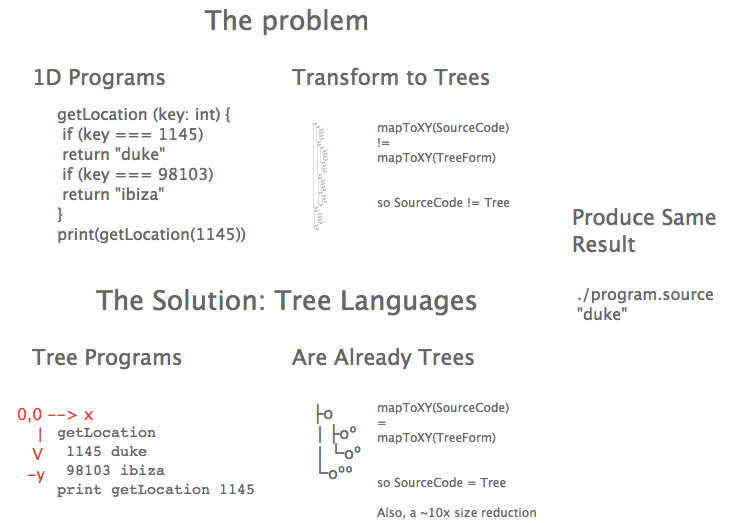
\includegraphics[width=90mm]{treenotation.png}
\caption{This diagram is the output of an ETN program.}
\end{figure}

\section{The Problem}

Programming is hard and complicated. Our current programming languages contribute a lot to this complexity. The standard approach to compiling code is to first transform that code into an Abstract Syntax Tree (AST). ASTs have enabled great gains in developer productivity. But programmers lose efficiencies and insight due to discrepancies between source code and ASTs.

\section{The Solution: Tree Notation}

In this paper and accompanying GitHub ES6 Repo (GER - github.com/breck7/treenotation), I introduce Tree Notation (TN), a new whitespace-based notation. You can extend TN to create domain specific languages (DSLs) that don't require a transformation to a discordant AST. These DSLs, called ETNs ("Extends Tree Notation"), are easy to create and can be simple or Turing Complete.

TN encodes one data structure, a \textbf{TreeNode}, with two members: a string called \textbf{line} and an optional array of child TreeNodes called \textbf{children}.

TN defines two special characters, which in the canonical notation are node delimiter ("\textbackslash n") and node edge (" "). Node edge is a space, not a tab. Many ETNs also use a space as a word delimiter.

A comparison quickly illustrates nearly the entirety of the notation:

JSON:

\begin{lstlisting}
{
 "title" : "Jack and Ada at BCHS",
 "visitors": {
  "mozilla": 802
 }
}
\end{lstlisting}

Tree Notation:

\begin{lstlisting}
title Jack and Ada at BCHS
visitors
 mozilla 802
\end{lstlisting}

\section{Useful Properties}

\subsection{Simplicity}

As shown in Fig 1, TN simply maps source code to an XY plane. Also, an ETN program uses far fewer source nodes than an equivalent program written in an Antique Language (AL).

\subsection{Zero parse errors}

Parse errors do not exist in TN. Every document is a valid TN document. Errors only exist at the ETN level (e.g., a mistyped word).

With most ALs, to get from a blank document to a certain valid document in keystroke increments requires stops at invalid documents. With TN all intermediate steps are valid.

A user can edit the nodes of a document at runtime with no risk of breaking the TN parsing of the entire document. If a node contains an ETN error, the ETN node interpreter can handle the error itself and even autocorrect itself.

A developer working on an editor that allows a user to edit source code does not have to worry about handling both errors at the DSL level and errors at the base notation level. TN eliminates the latter class of errors.

\subsection{Semantic diffs}

ALs can encode the same object to different documents by varying whitespace. Arbitrary whitespace is sometimes desirable. But programs often generate large diffs--and sometimes merge conflicts--for small or non-existent semantic changes.

In TN, editors have only one way to serialize a TN structure. Diffs contain only semantic meaning.

\subsection{Easy composition}

Base notations such as XML\cite{Bray}, JSON\cite{Crockford}, and Racket\cite{Racket} can encode multi-lingual documents. But to do that, those notations often complect those blocks.

In the example below, the program IPython encodes Python to JSON. The resulting document contains additional nodes:

\begin{lstlisting}
{
 "source": [
  "import hn.np as lz\n",
  "print(\"pdm\")"
  ]
}
\end{lstlisting}

With TN, the Python block is indented and requires no complecting:

\begin{lstlisting}
source
 import hn.np as lz
 print("pdm")
\end{lstlisting}

\section{Drawbacks}

\subsection{Lack of Tooling and Support}

TN is new, and library and application support, compared to other popular base notations, rounds to zero.

\subsection{Lack of Primitive Data Types in TN}

Some ALs have notations for common primitive types like floats and parse documents directly to efficient in-memory structures. "TN" is minimal so for best results, don't forget about "E" (to get "ETN").

The need for ETNs is a minor concern, as the GER demonstrates how useful ETNs can be built with just a few lines of code. And creating a TN library in other ALs is straightforward, and not comparable to the complexity of implementing a JSON library \cite{Ooms}, for example.

\subsection{Aesthetic Differences}

Without an ETN, TN can be verbose. A complex node in TN extends over multiple lines. ALs have a denser display of information out of the gate, with multiple nodes per line.

Other concerns have been raised. Some developers dislike space-indented notations, some wrongly prefer tabs, and some just have no taste.

\section{Predictions}

\textbf{Prediction 1: no structure will be found that cannot serialize to TN.} Some LISP programmers believe all data structures are recursive lists (or perhaps "recursive cons"). After seeing TN, I believe in The Tree Conjecture (TTC): \textbf{All structures are trees}.

For example, a hash table could serialize to HashTableETN:

\begin{lstlisting}
c 106
b 226
\end{lstlisting}

Therefore, hash tables are a type of tree. TTC stands.

\textbf{Prediction 2: Useful new ETNs may be found for every AL.} Below is some example code in a simple ETN, JsonETN.

\begin{lstlisting}
o
 s foundOn Sci-Hub
 n ma 902
\end{lstlisting}

ETNs will be found for great ALs including C, RISC-V, ES6, and Arc. Some ETNs have already been found \cite{Roughan}, but haven't been recognized as ETNs. The immediate benefit of discovering an ETN for an AL is that programs can then be written in an ETN editor and compiled to that AL.

\textbf{Prediction 3: Tree Oriented Programming (TOP) will replace Object Oriented Programming as the dominant architectural philosophy.} This will not surprise programmers who have experienced TOP (such as React developers).

\textbf{Prediction 4: The simplest 2D text encodings for neural networks will be ETNs.} High level ETNs will be found to transform massive GPU trained routines into understandable trees.

\section{Discovery Process and a call for Explorers}

TN was discovered by an iterative process, where the goal was to find a useful notation that aligns with certain geometric patterns. Perhaps an analogous process could be used for finding notations in higher dimensions.

The discovery of TN and ETNs will lead to new applications in visual programming, AI, VR/AR/Mobile programming, and more. I encourage you, the reader, to join in the exploration of this brave new world of programming languages!

\begin{figure}[ht!]
\centering
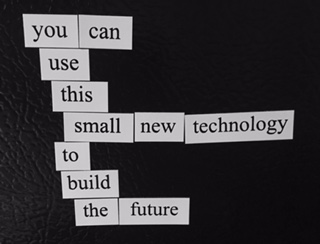
\includegraphics[width=90mm]{tree.jpg}
\caption{Rearranging these fridge magnets is equivalent to editing a TN document. The fridge magnet set that includes parentheses is a poor seller.}
\end{figure}

\begin{thebibliography}{4}

\bibitem{Bray}
Bray, Tim, et al. "Extensible markup language (XML)." World Wide Web Consortium Recommendation REC-xml-19980210. http://www. w3. org/TR/1998/REC-xml-19980210 16 (1998): 16.

\bibitem{Crockford}
Crockford, Douglas. "The application/json media type for javascript object notation (json)." (2006).

\bibitem{Racket}
Tobin-Hochstadt, Sam, et al. "Languages as libraries." ACM SIGPLAN Notices. Vol. 46. No. 6. ACM, 2011.

\bibitem{Ooms}
Ooms, Jeroen. "The jsonlite package: A practical and consistent mapping between json data and r objects." arXiv preprint arXiv:1403.2805 (2014).

\bibitem{Roughan}
Roughan, Matthew, and Jonathan Tuke. "Unravelling graph-exchange file formats." arXiv preprint arXiv:1503.02781 (2015).

\end{thebibliography}

\ifCLASSOPTIONcaptionsoff
  \newpage
\fi

\end{document}
